% ==== DISCRIMINATING AGAINST QCD Zy PRODUCTION SECTION ====

The biggest challenge in this analysis is managing the dominant background,
\ac{QCD} \Zyjj production. Like the signal process, this background has a real Z
boson and photon. The difference is the origin of the jets, here not from a
boson decay but more likely radiated from the initial or final state.
%
Identifying and exploiting the differences in jet kinematics between this
background and the signal is therefore key to maximising the sensitivity of the
measurement. This section is dedicated to discussing this problem; thus here the
word signal is used to refer to \ac{EW} V\Zy production and background refers
solely to \ac{QCD} \Zyjj production.

%TODO give Feynman diagrams? Or reference previous Feynmans

% Talk about kinematic differences
There are a small number of kinematic distributions which exhibit a large
difference between signal and background that could be exploited effectively by
a cut; the dijet mass, $m_{jj}$, being an obvious example as for the signal it
peaks around the W/Z boson mass but for the background resembles a continuum.
For a great many more variables however, the differences are more subtle. Whilst
there is frequently an obvious difference in shape between signal and
background, there is no obvious set of cuts that would create a signal-rich
region. Figure \ref{fig:vzy-bdt-ewvqcd} shows some distributions with the
largest signal-background discrepancies.

% m_jj and cos_theta_CS_jj show cuttable differences

\begin{figure}
  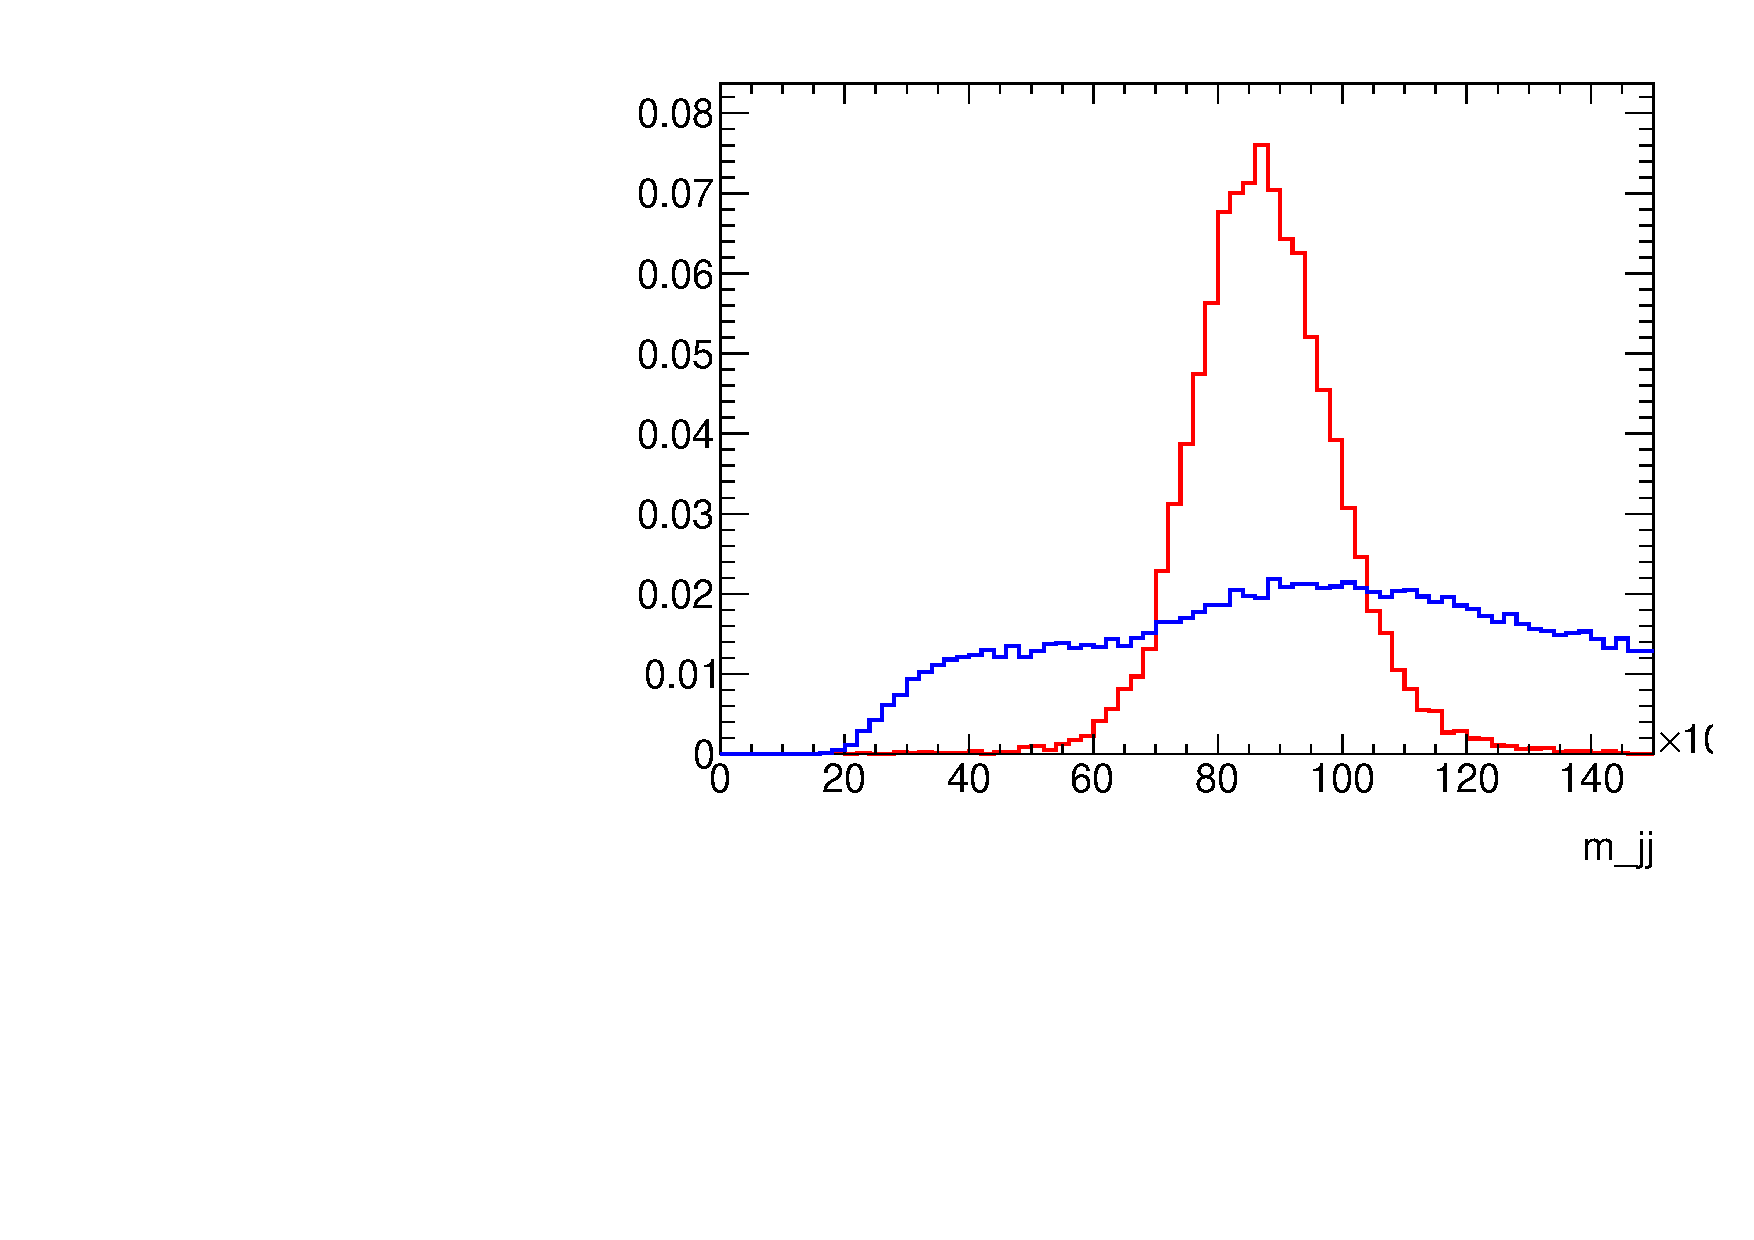
\includegraphics[width=.49\textwidth]{\resource{EWvQCD/m_jj.pdf}}
  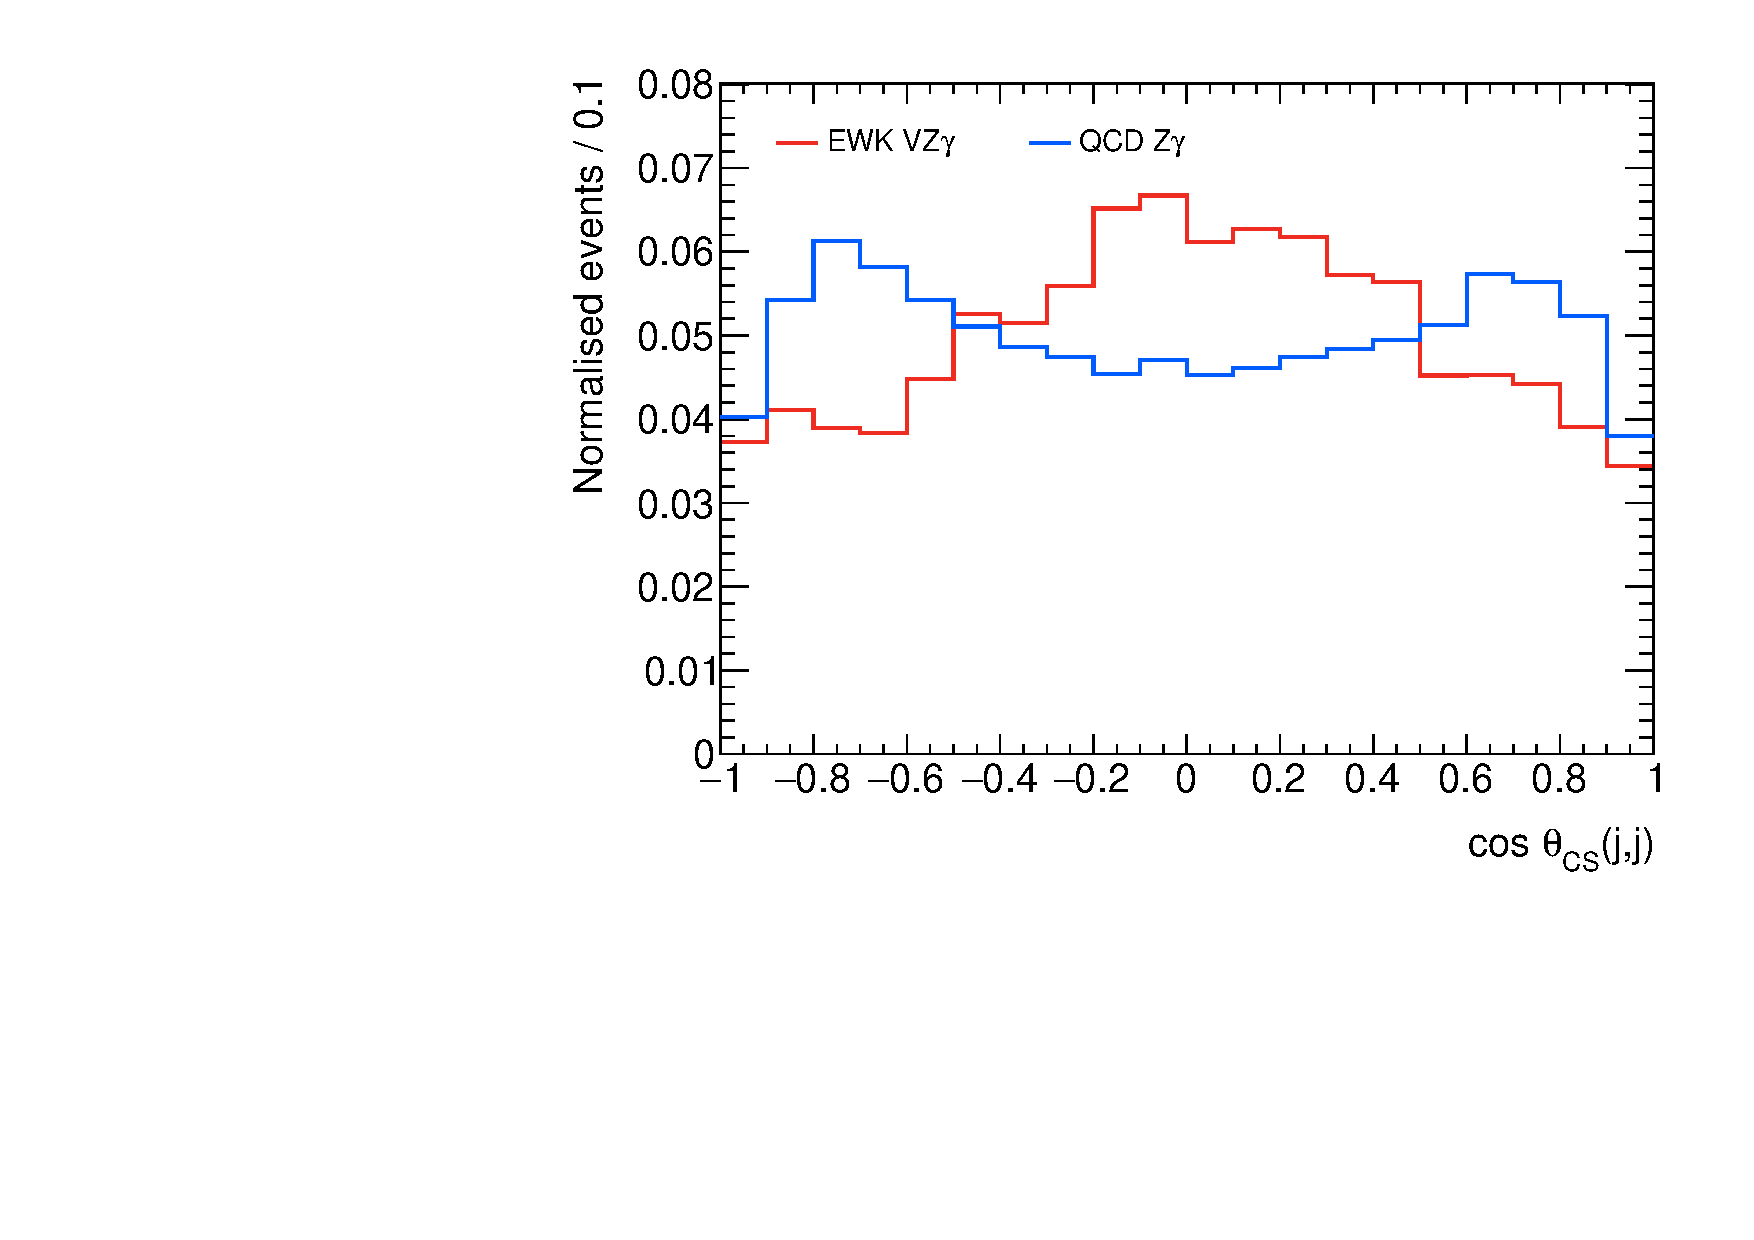
\includegraphics[width=.49\textwidth]{\resource{EWvQCD/cos_theta_CS_jj.pdf}}
  \\
  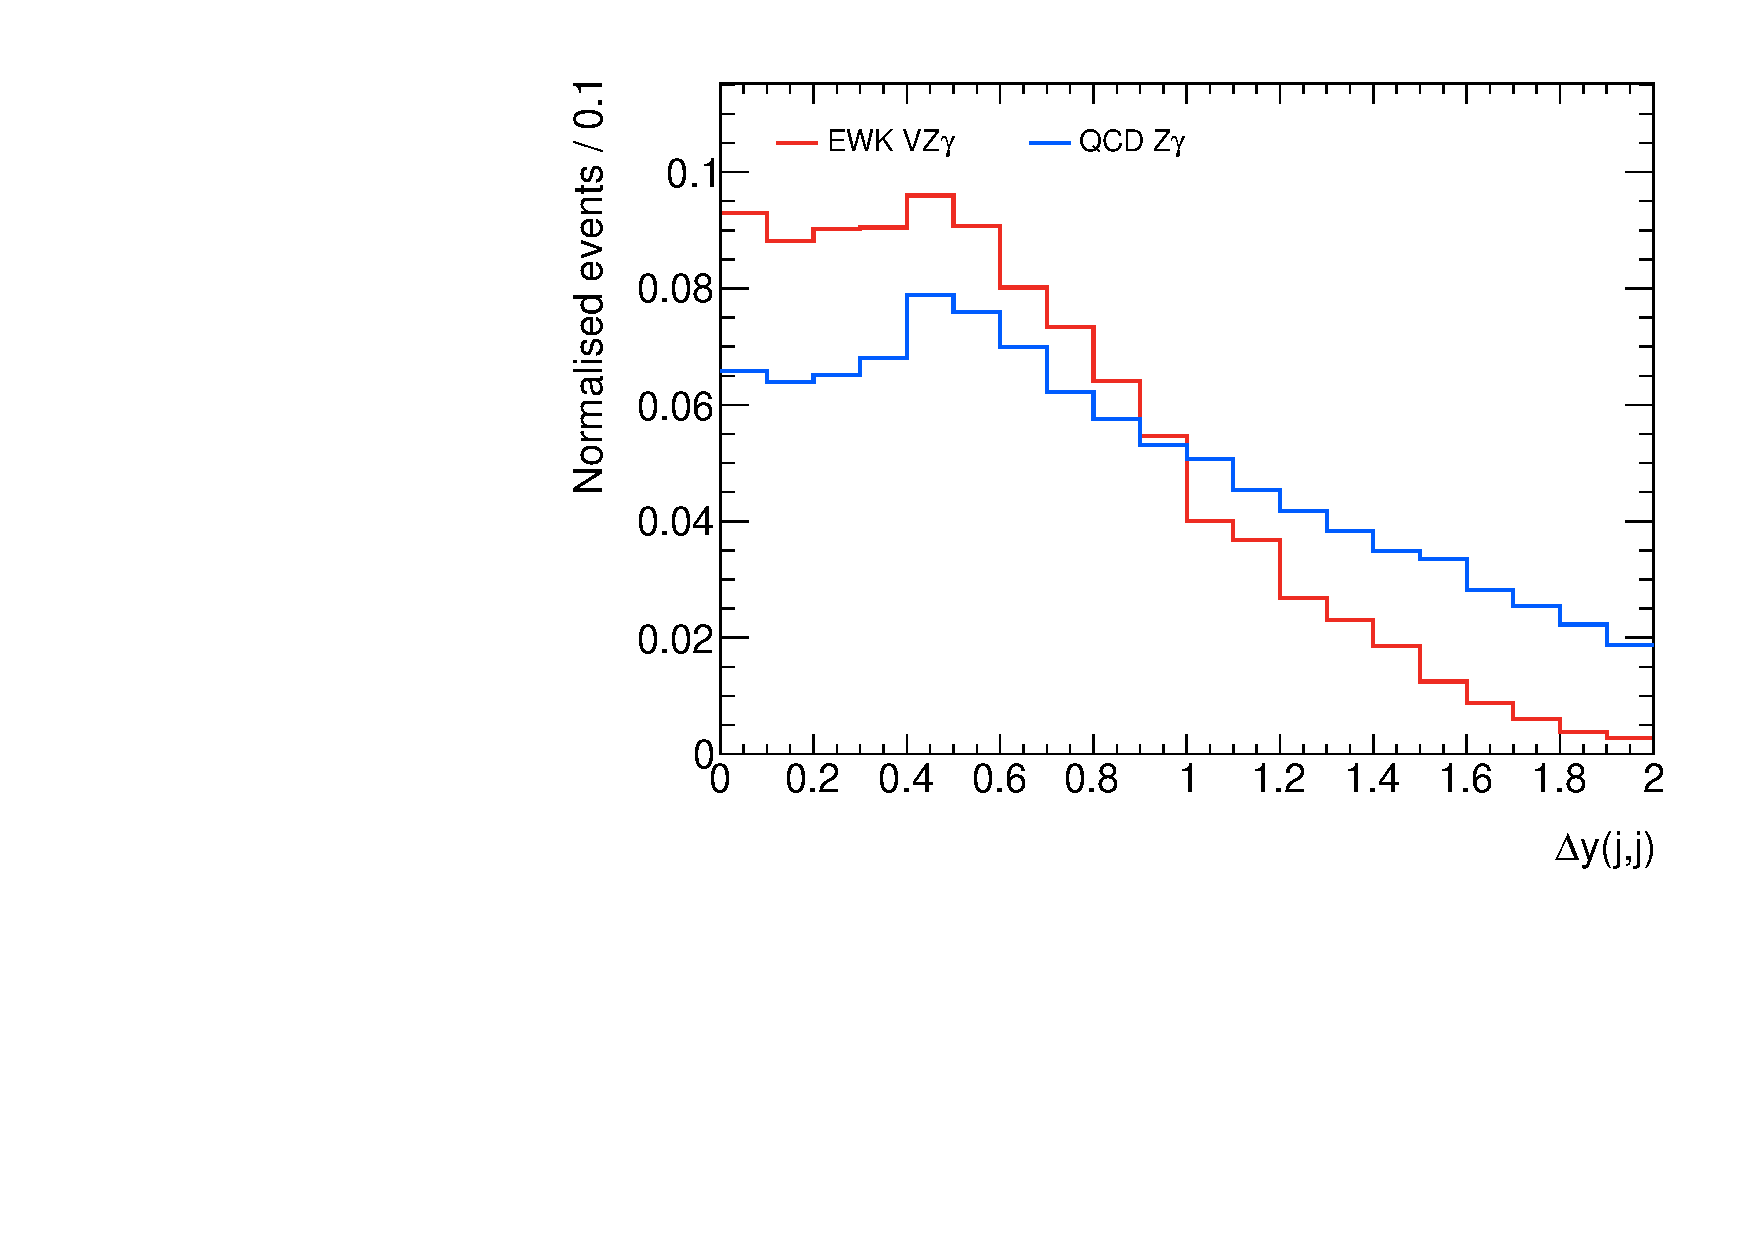
\includegraphics[width=.49\textwidth]{\resource{EWvQCD/Dy_j_j.pdf}}
  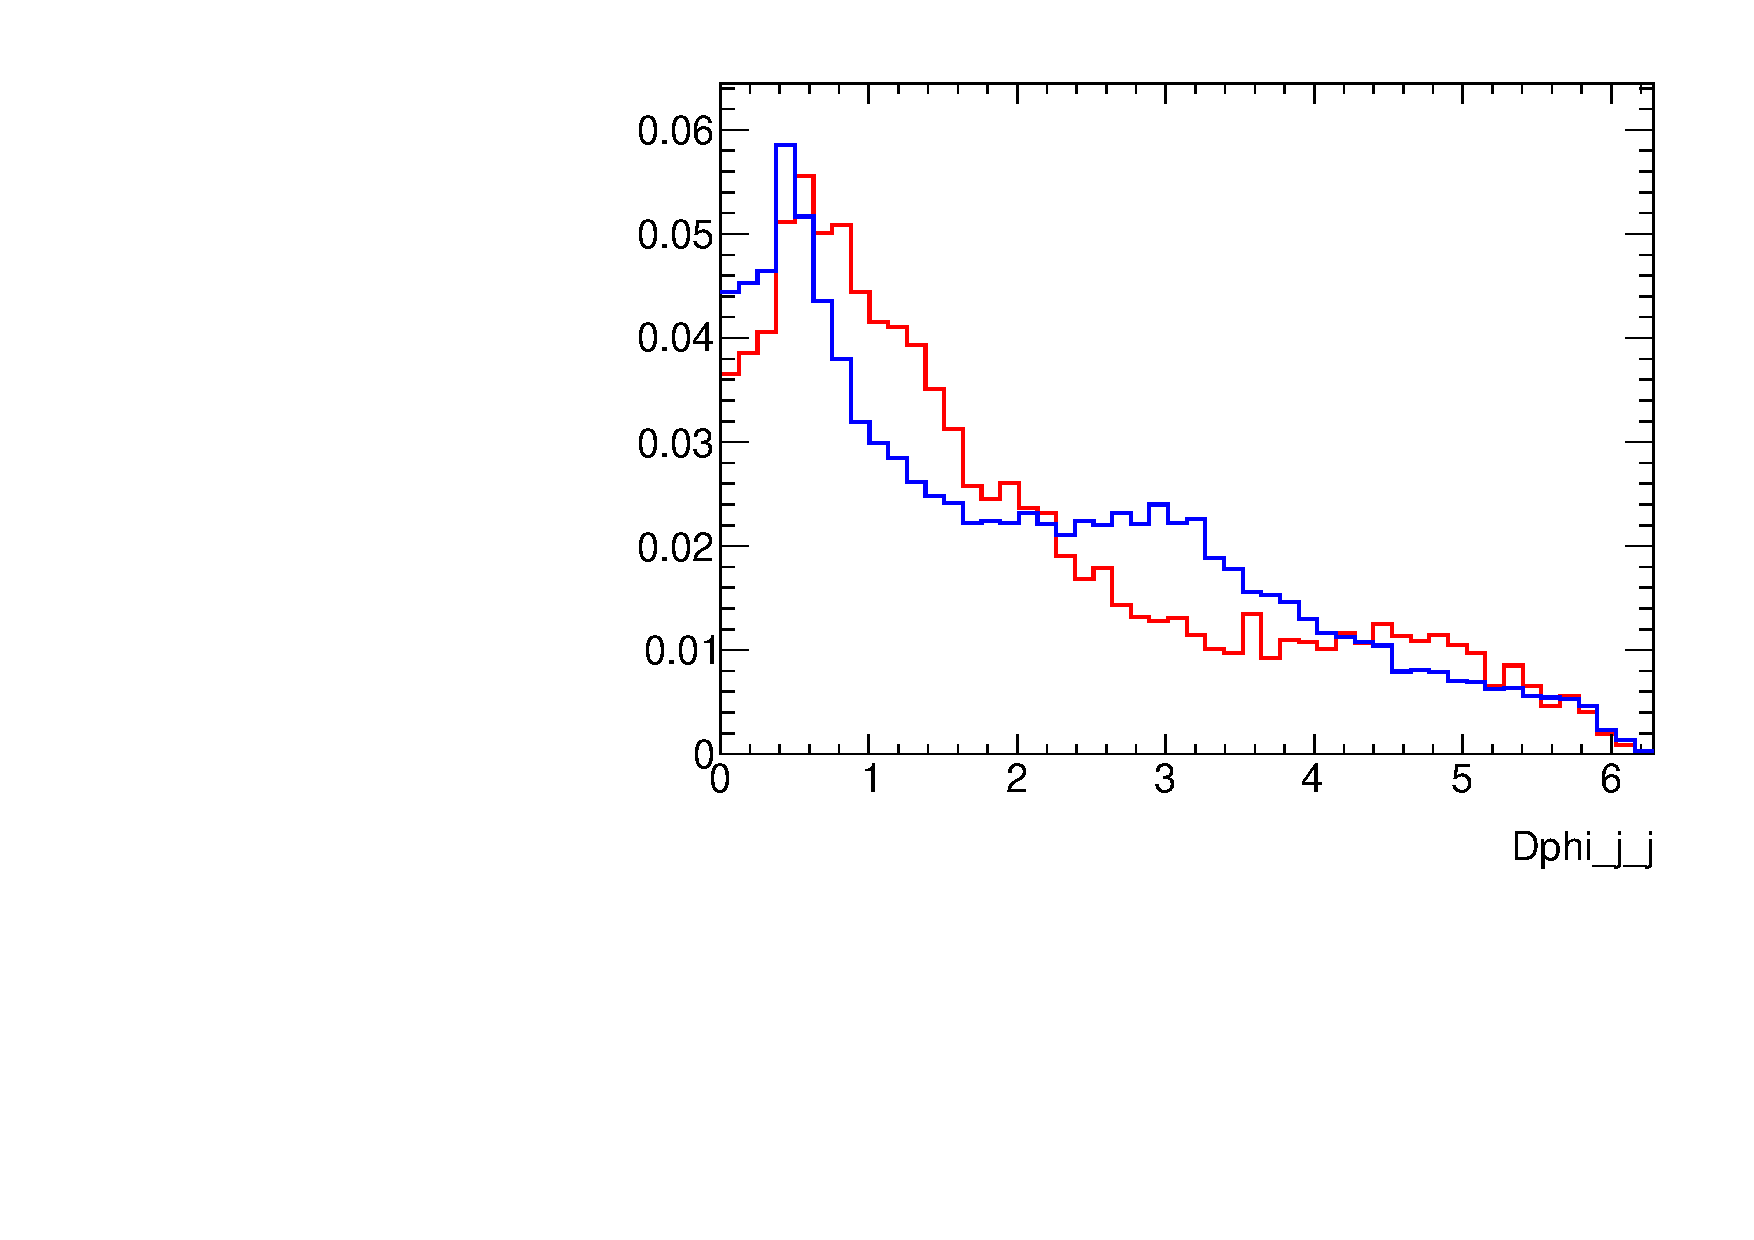
\includegraphics[width=.49\textwidth]{\resource{EWvQCD/Dphi_j_j.pdf}}
  \\
  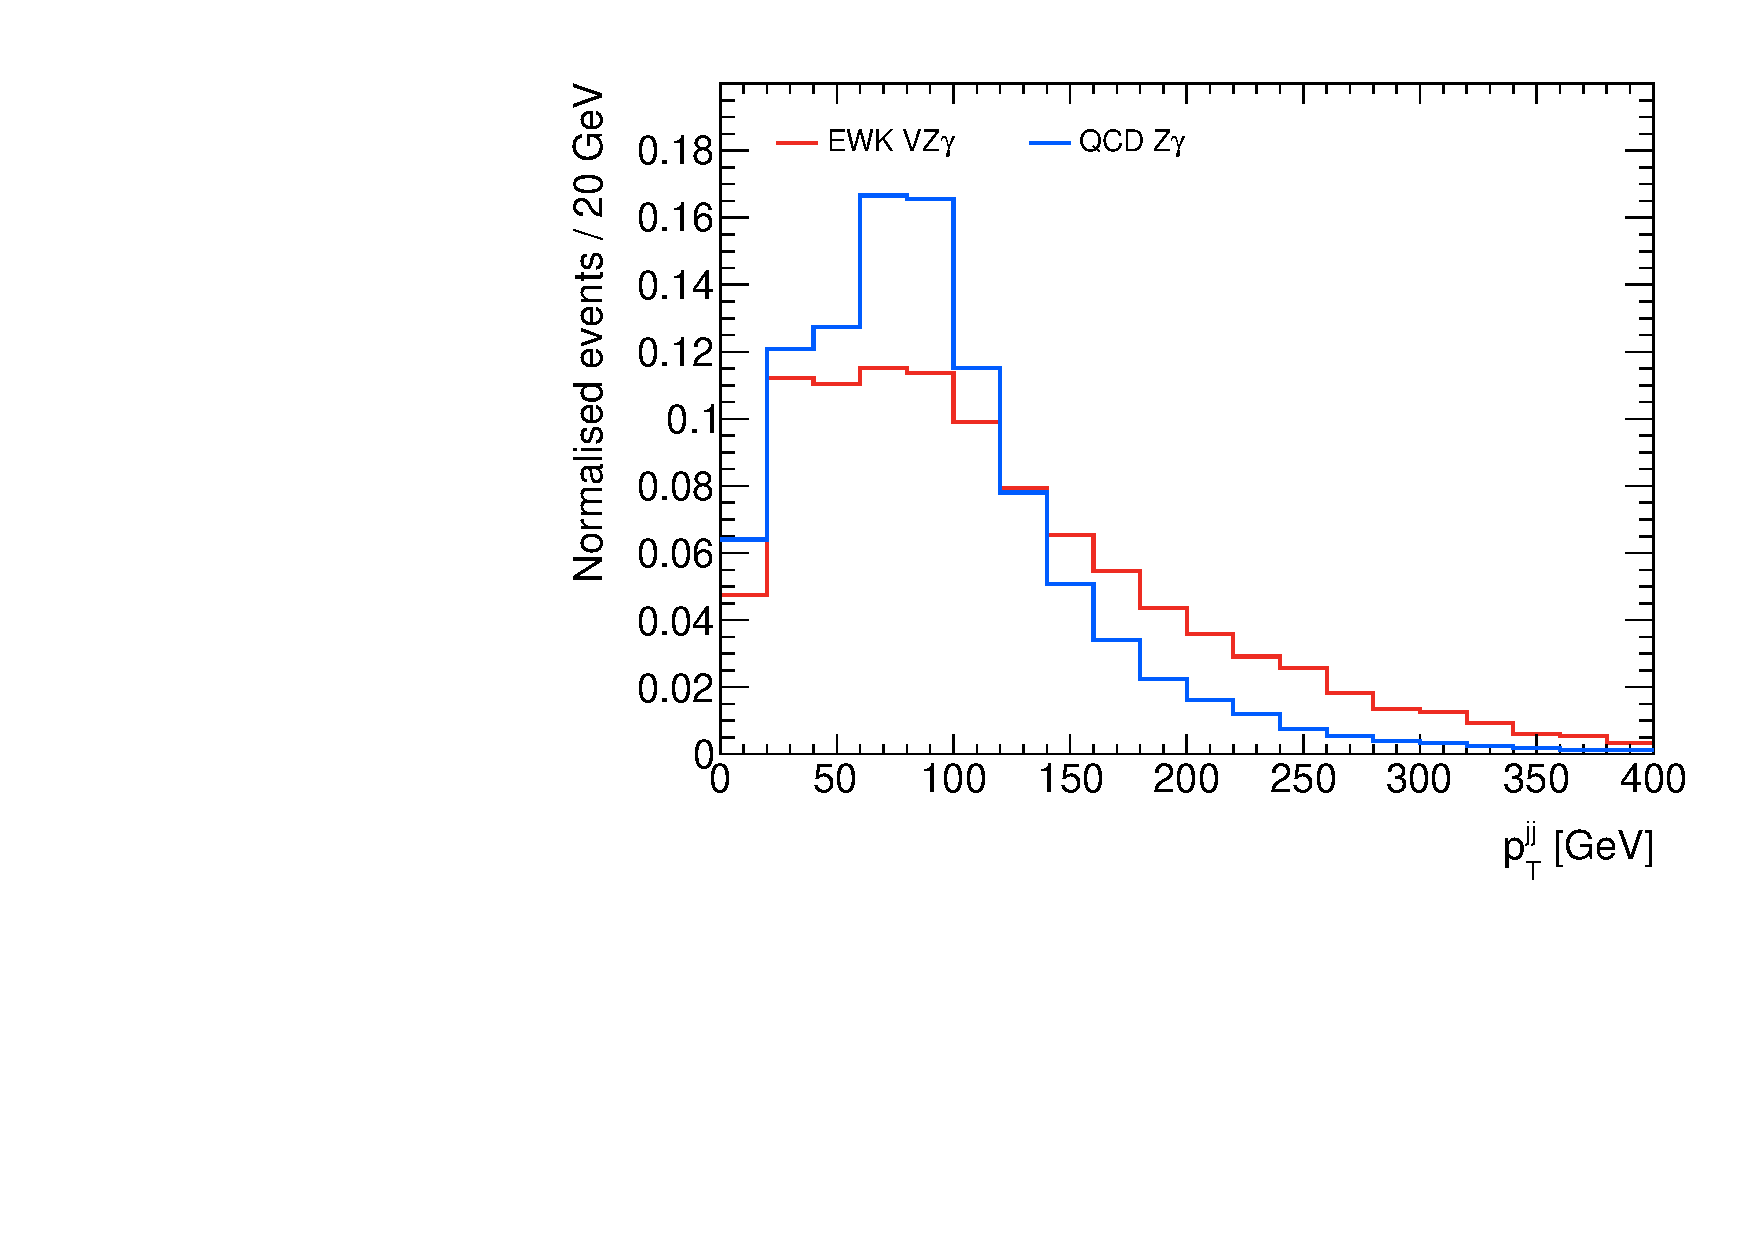
\includegraphics[width=.49\textwidth]{\resource{EWvQCD/pT_jj.pdf}}
  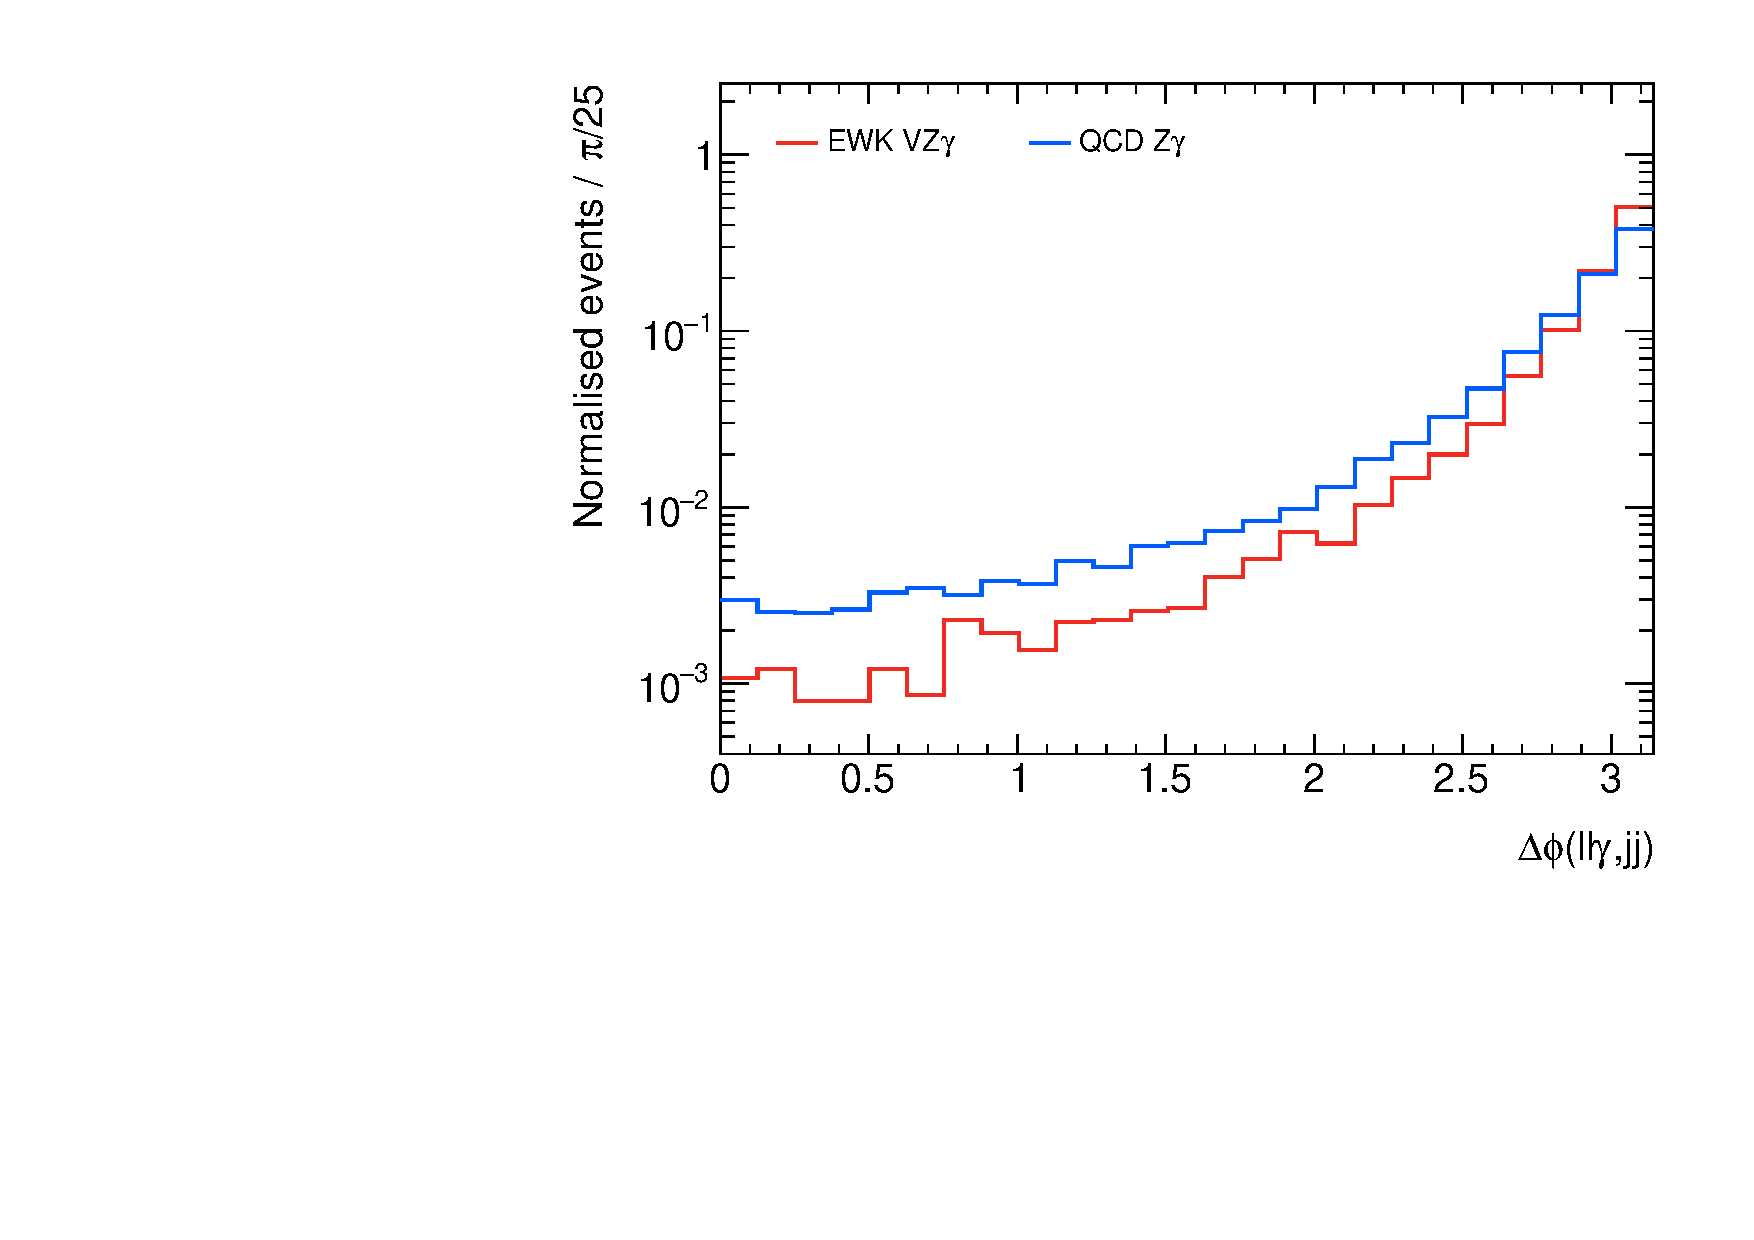
\includegraphics[width=.49\textwidth]{\resource{EWvQCD/Dphi_lly_jj.pdf}}
  %
  \caption{
    Kinematic distributions, comparing \acs{EW} V\Zy production (red) to \acs{QCD}
    \Zyjj production (blue).
    [Placeholder plots, to be updated] %TODO
  }
  \label{fig:vzy-bdt-ewvqcd}
\end{figure}
